% Options for packages loaded elsewhere
\PassOptionsToPackage{unicode}{hyperref}
\PassOptionsToPackage{hyphens}{url}
%
\documentclass[
]{article}
\usepackage{amsmath,amssymb}
\usepackage{iftex}
\ifPDFTeX
  \usepackage[T1]{fontenc}
  \usepackage[utf8]{inputenc}
  \usepackage{textcomp} % provide euro and other symbols
\else % if luatex or xetex
  \usepackage{unicode-math} % this also loads fontspec
  \defaultfontfeatures{Scale=MatchLowercase}
  \defaultfontfeatures[\rmfamily]{Ligatures=TeX,Scale=1}
\fi
\usepackage{lmodern}
\ifPDFTeX\else
  % xetex/luatex font selection
\fi
% Use upquote if available, for straight quotes in verbatim environments
\IfFileExists{upquote.sty}{\usepackage{upquote}}{}
\IfFileExists{microtype.sty}{% use microtype if available
  \usepackage[]{microtype}
  \UseMicrotypeSet[protrusion]{basicmath} % disable protrusion for tt fonts
}{}
\makeatletter
\@ifundefined{KOMAClassName}{% if non-KOMA class
  \IfFileExists{parskip.sty}{%
    \usepackage{parskip}
  }{% else
    \setlength{\parindent}{0pt}
    \setlength{\parskip}{6pt plus 2pt minus 1pt}}
}{% if KOMA class
  \KOMAoptions{parskip=half}}
\makeatother
\usepackage{xcolor}
\usepackage{graphicx}
\makeatletter
\newsavebox\pandoc@box
\newcommand*\pandocbounded[1]{% scales image to fit in text height/width
  \sbox\pandoc@box{#1}%
  \Gscale@div\@tempa{\textheight}{\dimexpr\ht\pandoc@box+\dp\pandoc@box\relax}%
  \Gscale@div\@tempb{\linewidth}{\wd\pandoc@box}%
  \ifdim\@tempb\p@<\@tempa\p@\let\@tempa\@tempb\fi% select the smaller of both
  \ifdim\@tempa\p@<\p@\scalebox{\@tempa}{\usebox\pandoc@box}%
  \else\usebox{\pandoc@box}%
  \fi%
}
% Set default figure placement to htbp
\def\fps@figure{htbp}
\makeatother
\setlength{\emergencystretch}{3em} % prevent overfull lines
\providecommand{\tightlist}{%
  \setlength{\itemsep}{0pt}\setlength{\parskip}{0pt}}
\setcounter{secnumdepth}{-\maxdimen} % remove section numbering
\usepackage{bookmark}
\IfFileExists{xurl.sty}{\usepackage{xurl}}{} % add URL line breaks if available
\urlstyle{same}
\hypersetup{
  hidelinks,
  pdfcreator={LaTeX via pandoc}}

\author{}
\date{}

\begin{document}

\subsection{第2章
MOS器件物理基础}\label{ux7b2c2ux7ae0ux9mosux5668ux4ef6ux7269ux7406ux57faux7840}

\paragraph{学习集成电路设计的一些思路:}\label{ux5b66ux4e60ux96c6ux6210ux7535ux8defux8bbeux8ba1ux7684ux4e00ux4e9bux601dux8def}

(热学+电磁学 \(\longrightarrow\) )量子力学 \(\longrightarrow\)
固体物理、半导体物理、器件物理 \(\longrightarrow\) 电路设计

将半导体器件看作黑盒子,只关注伏安特性曲线在电路中的运用

\paragraph{\texorpdfstring{\(MOSFET\)
基本介绍}{MOSFET 基本介绍}}\label{mosfetuxa-ux57faux672cux4ecbux7ecd}

\pandocbounded{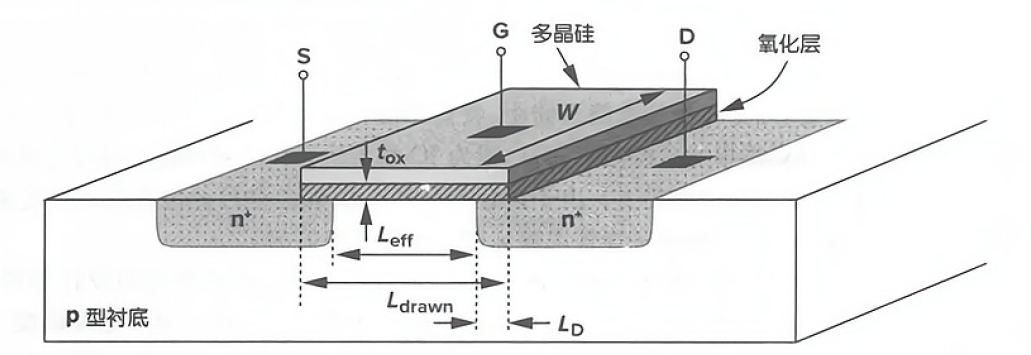
\includegraphics[keepaspectratio]{https://raw.githubusercontent.com/heiheiha798/Razavi-Notes/main/img/image-20240709000742746.png}}

\(Metal-Oxide-Semiconductor\ Field-Effect\ Transistor\)

四端器件:栅、源、漏、衬 ( \(Gate、Source、Drain、Bulk\) )

源:提供载流子的终端

漏:收集载流子的终端

重要尺寸:源漏通道的横向尺寸栅长 \(L\) ,垂直方向栅宽 \(W\) ,氧化层厚度
\(t_{ox}\) ,

典型工作时 \(GD\) 二极管反偏,所以 \(n\) 阱往往接高电位

\(MOS\) 符号:

\pandocbounded{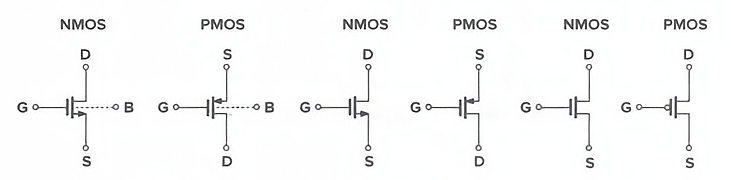
\includegraphics[keepaspectratio]{https://raw.githubusercontent.com/heiheiha798/Razavi-Notes/main/img/image-20240709001959403.png}}

NMOS和PMOS器件的衬底端通常接地和接 \(V_{DD}\) ,所以通常省略 \(B\) 端

\paragraph{\texorpdfstring{\(MOS\) 的 \(I-V\)
特性}{MOS 的 I-V 特性}}\label{mosuxa-ux7684-uxaiux2212vuxa-ux7279ux6027}

以 \(NMOS\) 为例

阈值电压 \(V_{TH}\) :通常定义为界面的少子浓度等于多子浓度时的栅压

\[V_{TH}=\Psi_{MS}+2\Psi_F+\frac{Q_{dep}}{C_{ox}}\]

\(\Psi_{MS}\) 是多晶硅栅和硅衬底的功函数差电压值

\(\Psi_{F}=\frac{kT}{q}ln(\frac{N_{sub}}{n_i})\) ,其中 \(N_{sub}\)
是衬底掺杂浓度, \(n_i\) 是硅本征载流子浓度

\(Q_{dep}\) 是耗尽区电荷(
\(Q_{dep}=\sqrt{4 q \varepsilon_{si} |\Psi_{F}|N_{sub}}\) )

\(C_{ox}\) 是单位面积的栅氧化层的电容

制造中往往在沟道区注入杂质调整阈值电压

\begin{equation}
\begin{split}
Q_{d} &= WC_{ox}(V_{GS}-V_{TH})\\\Rightarrow
Q_{d}(x) &= WC_{ox}[V_{GS}-V(x)-V_{TH}]\\\Rightarrow
I_{D} &= -WC_{ox}[V_{GS}-V(x)-V_{TH}]v\\\Rightarrow
I_{D} &= WC_{ox}[V_{GS}-V(x)-V_{TH}]\mu_{n}\frac{dV(x)}{dx}\\\Rightarrow
\int_{x=0}^{L} I_{D}dx &= \int_{V=0}^{V_{DS}}WC_{ox}\mu_{n}[V_{GS}-V(x)-V_{TH}]dV\\\Rightarrow
I_{D} &= \mu_{n}C_{ox}\frac{W}{L}[(V_{GS}-V_{TH})V_{DS}-\frac{1}{2}V_{DS}^2]
\end{split}
\end{equation}

称 \(V_{GS}-V_{TH}\) 为过驱动电压, \(\frac{W}{L}\) 为宽长比

注意:这里的积分上限是
\(L\),这意味着我们默认沟道全导通,这让我们得到了一个抛物线

在抛物线的起始区域做线性近似,得到

\[I_D \approx \mu_{n}C_{ox}\frac{W}{L}(V_{GS}-V_{TH})V_{DS}\]

这意味着我们可以将 \(MOS\) 器件看作一个压控线性电阻,这段称为``欧姆区''

考虑 \(V_{GS}\) 比较大,超过抛物线的极值点,即 \(V_{DS}>V_{GS}-V_{TH}\)
时,注意到

\[Q_{d}(x) = WC_{ox}[V_{GS}-V(x)-V_{TH}]\]

这意味某些区域中少子浓度太低,还处在耗尽状态,这导致沟道被夹断,其长度小于
\(L\) ,这将改变积分的上限

\begin{equation}
\begin{split}
\int_{x=0}^{L'} I_{D}dx &= \int_{V=0}^{V_{GS}-V_{TH}}WC_{ox}\mu_{n}[V_{GS}-V(x)-V_{TH}]dV\\\Rightarrow
I_{D}L' &= \frac{1}{2}WC_{ox}\mu_{n}(V_{GS}-V_{TH})^2\\\Rightarrow
I_{D} &= \frac{1}{2}\frac{W}{L'}C_{ox}\mu_{n}(V_{GS}-V_{TH})^2
\end{split}
\end{equation}

若忽略 \(L'\) 和 \(L\)
的差别,则器件的电流恒定,成为压控流源,这段称为``饱和区''

对于 \(PMOS\) 器件,只需将所有有正负意义的物理量取反即可

综上推导:\pandocbounded{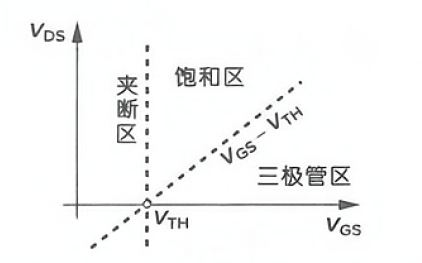
\includegraphics[keepaspectratio]{https://raw.githubusercontent.com/heiheiha798/Razavi-Notes/main/img/image-20240709093424846.png}}

\end{document}
